\documentclass[a4j]{jarticle}
\usepackage[dvipdfmx]{graphicx}
\usepackage{subfig}

\renewcommand{\labelenumi}{(\arabic{enumi})}

\title{中間報告書(1) \\ A班}
\author{秋元淳矢 \and 天笠智哉 \and 小林広人}
\date{}

\begin{document}

\maketitle

\section{現在の状況}
\subsection{完成した機能}
現在、完成している機能を以下に示す。
\begin{description}
	\item[WishListのメイン画面] \mbox{}
		\begin{description}
			\item[1. Model] \mbox{} \\
				WishListのModelは主に欲しいもののデータ(ID,名前,値段,予定日,購入状況)のリスト、リストのソートなどを含む編集機能のロジックを実装した。
			\item[2. ViewModel] \mbox{} \\
				WishListのViewModelはReactivePropertyを用いることで簡潔なViewとModelの仲介を実装することができた。
				ViewModelではページ遷移時の処理、昇順降順変更による再ソート呼び出し、ソート方法の変更による再ソート呼び出しなどを実装した。
			\item[3. View] \mbox{} \\
				WishListのViewは主にXamarinの1つの機能であるListViewを用いて実装を行った。また昇順降順ボタン,ソート方法を変更できるPickerも実装した。
		\end{description}
		以下にAndroid、UWPでのWishListの画面を示す。
		\begin{figure}[htbp]
			\centering
			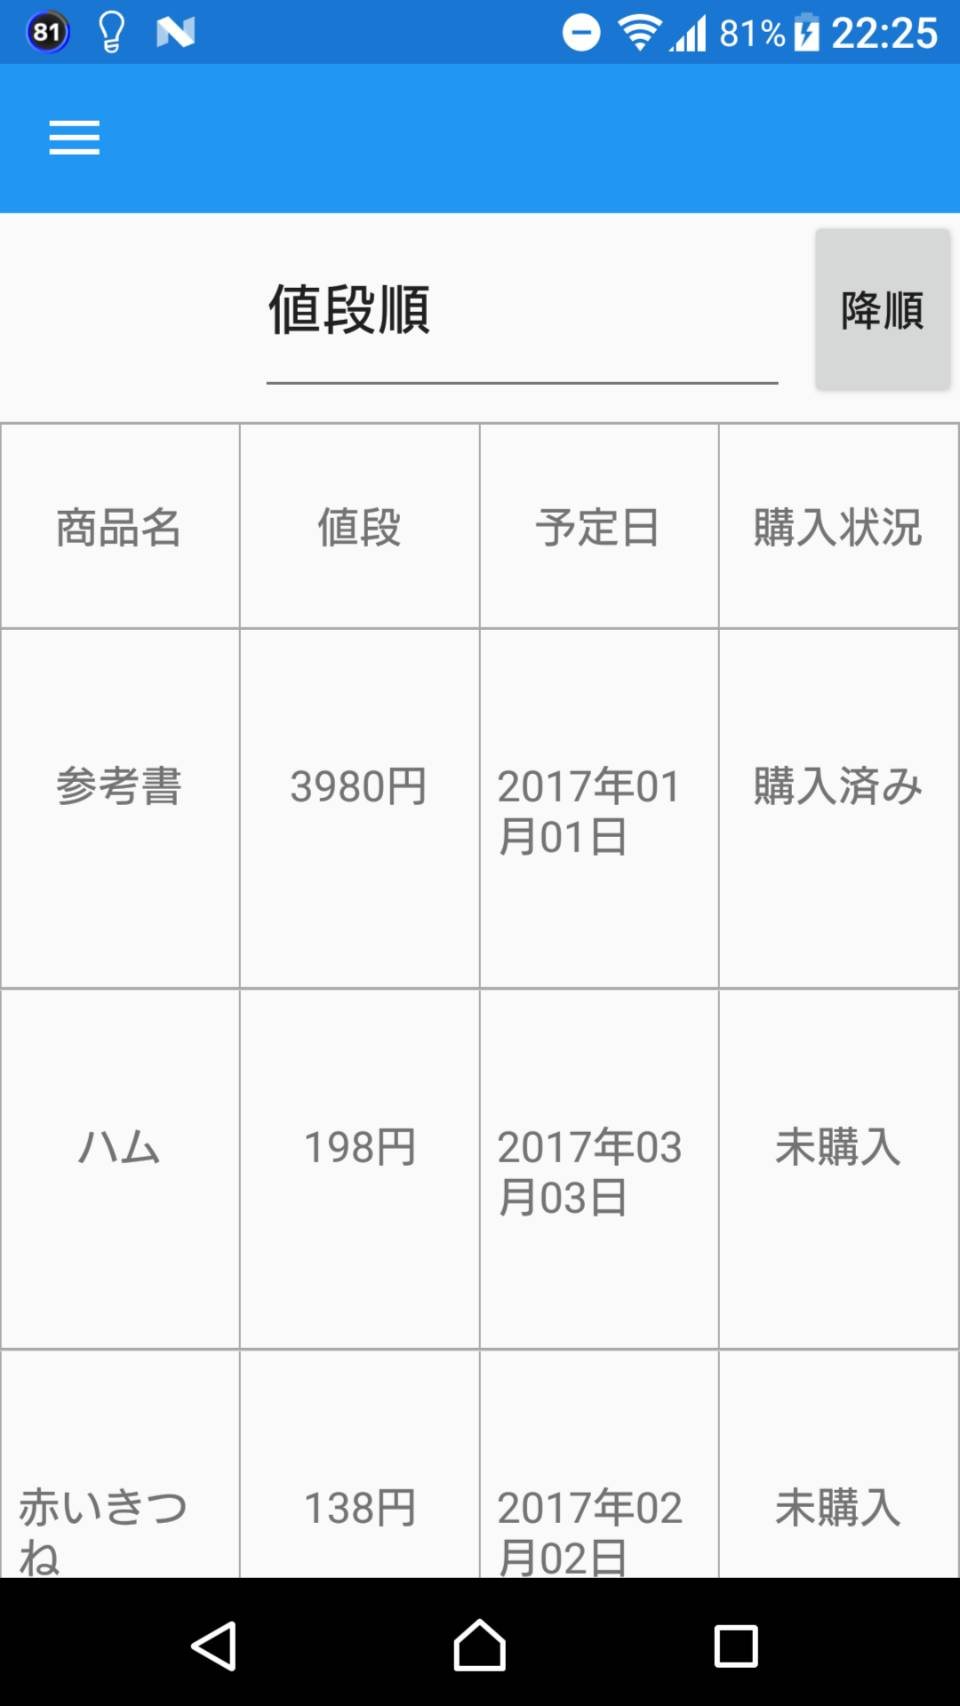
\includegraphics[width=100mm]{figures/WishListMainAndroid.jpg}
			\caption{Androidの環境でWishListを表示したときの画面図}
			\label{WishListMainFig1}
		\end{figure}
		\begin{figure}[htbp]
			\centering
			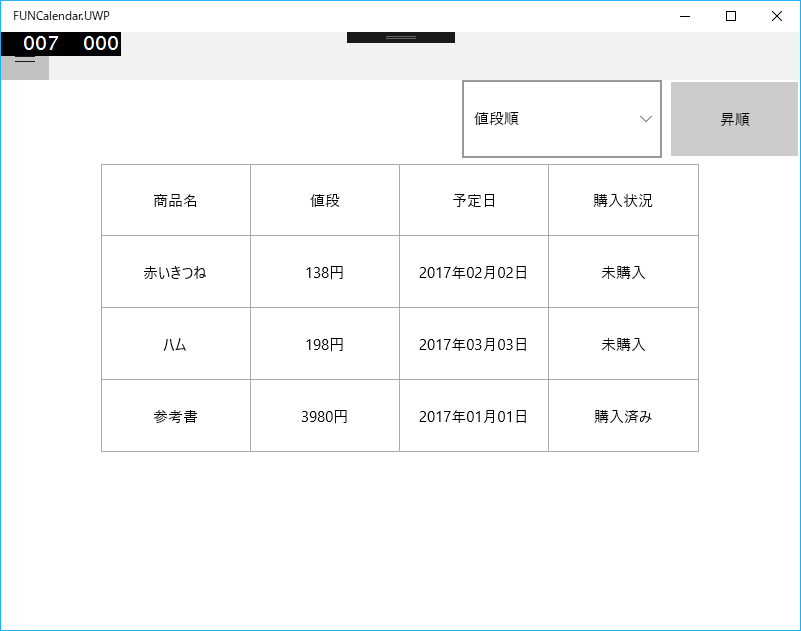
\includegraphics[height=120mm]{figures/WishListMainUWP.png}
			\caption{UWPの環境でWishListを表示したときの画面図}
			\label{WishListMainFig2}
		\end{figure}
		\clearpage

	\item[Menu] \mbox{} \\
		図\ref{MenuFig1}にAndroidの環境でmenuを表示したときの画面を示す。
		画面左端からのスワイプで表示されるMenuをMasterDetailPageを使うことで実装した。
		Menuの項目はCalendar,ToDo,WishList,家計簿の4つで、項目を押すとそれぞれの画面に遷移する。
		\begin{figure}[htbp]
			\centering
			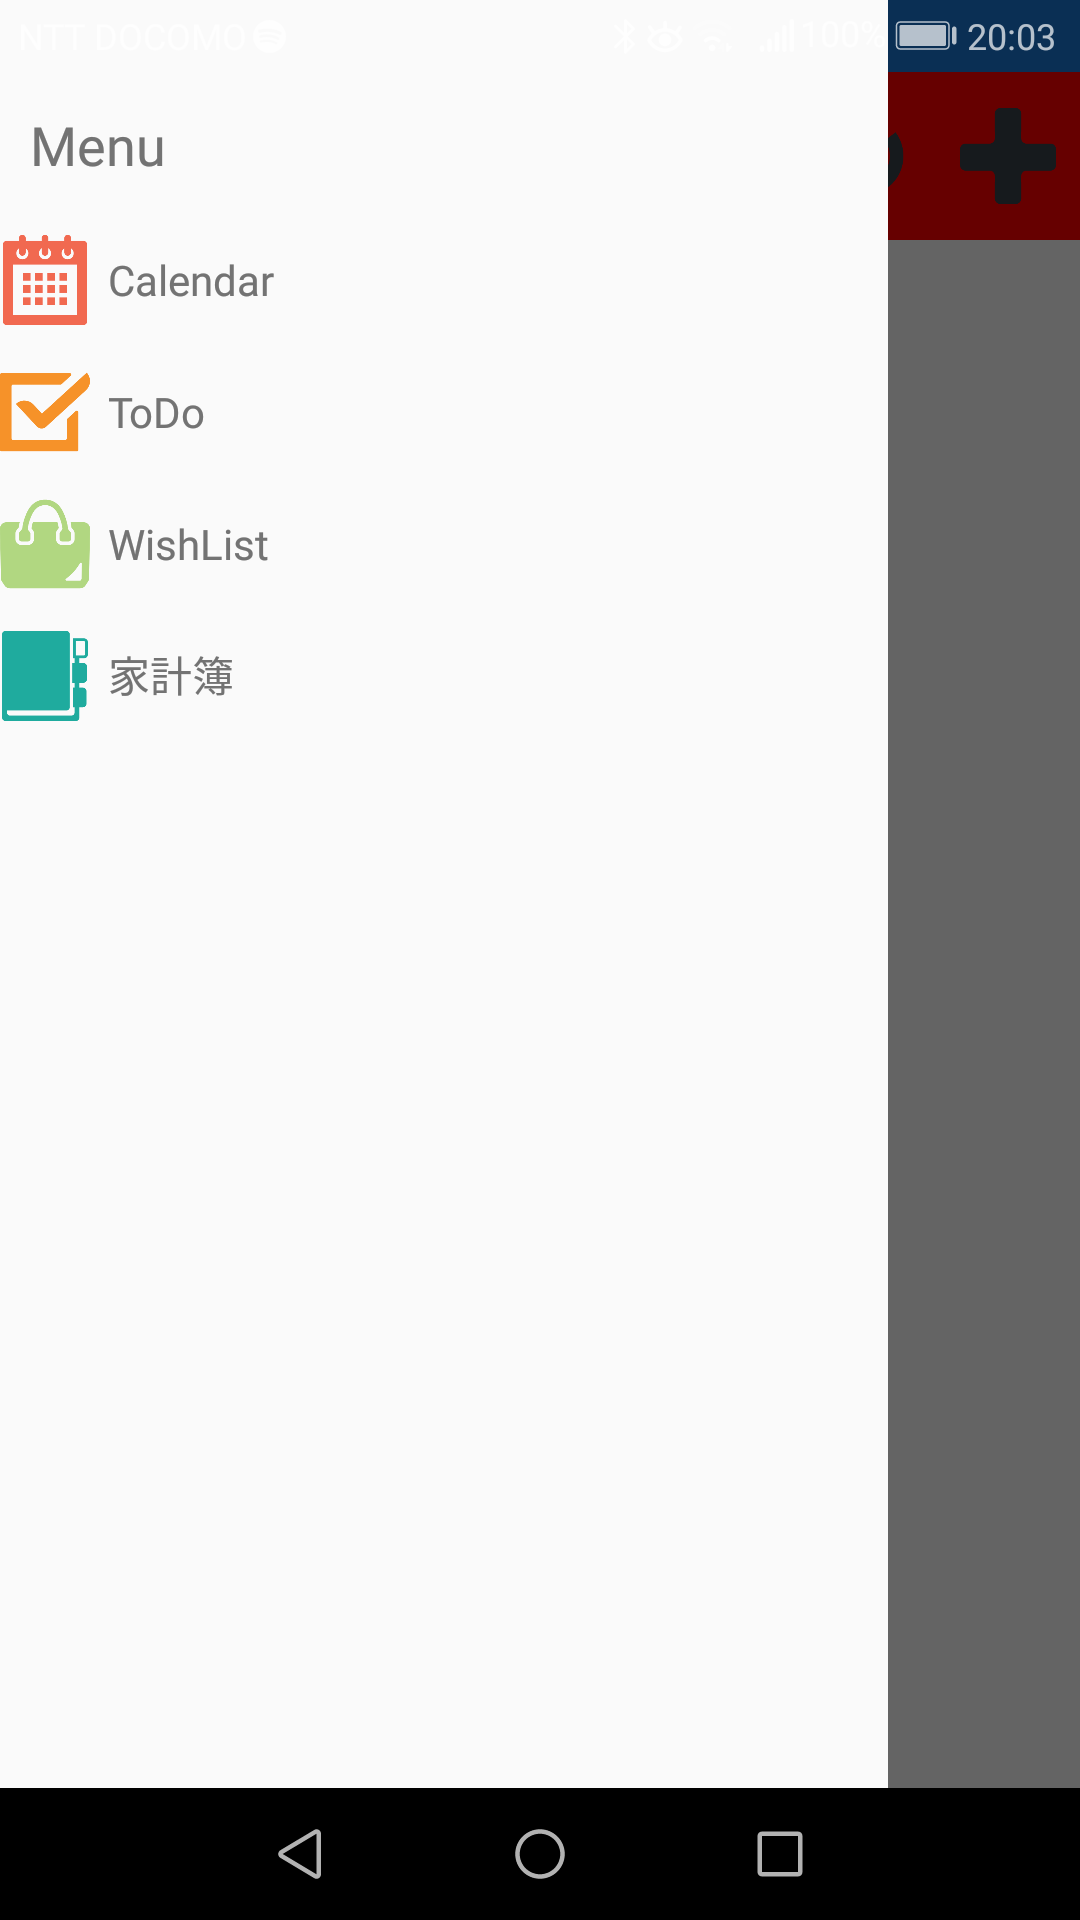
\includegraphics[width=90mm]{figures/MenuPage.png}
			\caption{Androidの環境でmenuを表示したときの画面図}
			\label{MenuFig1}
		\end{figure}
\end{description}
\clearpage

\subsection{開発中の機能}
現在開発中の機能を以下に示す。
\begin{description}
	\item[CalenderのModel] \mbox{} \\
		CalenderのModelはWishlist,ToDo,家計簿と関わりがあるため、完成させるには他の機能が完成する必要がある。
		現在、Calender単体としてのModelはほぼ完成している。
		そのため、CalenderのModelを完成させるには少しプログラムを変更すれば良い。
		CalenderのView,ViewModelを作成しつつ、Modelを完成させる予定だ。
\end{description}

\section{今後の課題}
現在のWishListは表示された画面があまり見やすくない。
色を付けるなどして画面の見やすさを追求し、今後のプログラム作成を続けていきたい。

\section{補足}
仕様書の説明が不十分である点が数か所見受けられた。
以下に追加する補足説明を示す。
\begin{description}
	\item[WishList] \mbox{} \\
		WishListで表示する項目が明記されていなかったため、表示する項目を改めて示す。
		表示する項目は、商品名、値段、予定日、購入状況の4つである。
		表示しない項目は、IDの1つである。
	\item[ToDo] \mbox{} \\
		ToDoで表示する項目が明記されていなかったため、表示する項目を改めて示す。
		表示する項目は、内容、日付、優先度、完了かどうかの4つである。
		表示しない項目は、ID、WishListのIDの2つである。
\end{description}

\end{document}